\section{Double-slit patterns}\label{sec:Double slit}
According to the theory we used, the intensity for double slit patterns can be approximated as:
\begin{aligned}
    I(x)=\frac{kd^2\cos^2\left(\frac{kLx}{2z}\right)sinc^2\left(\frac{dkx}{2z}\right)}{\pi z}
\end{aligned}

\begin{figure}[H]
    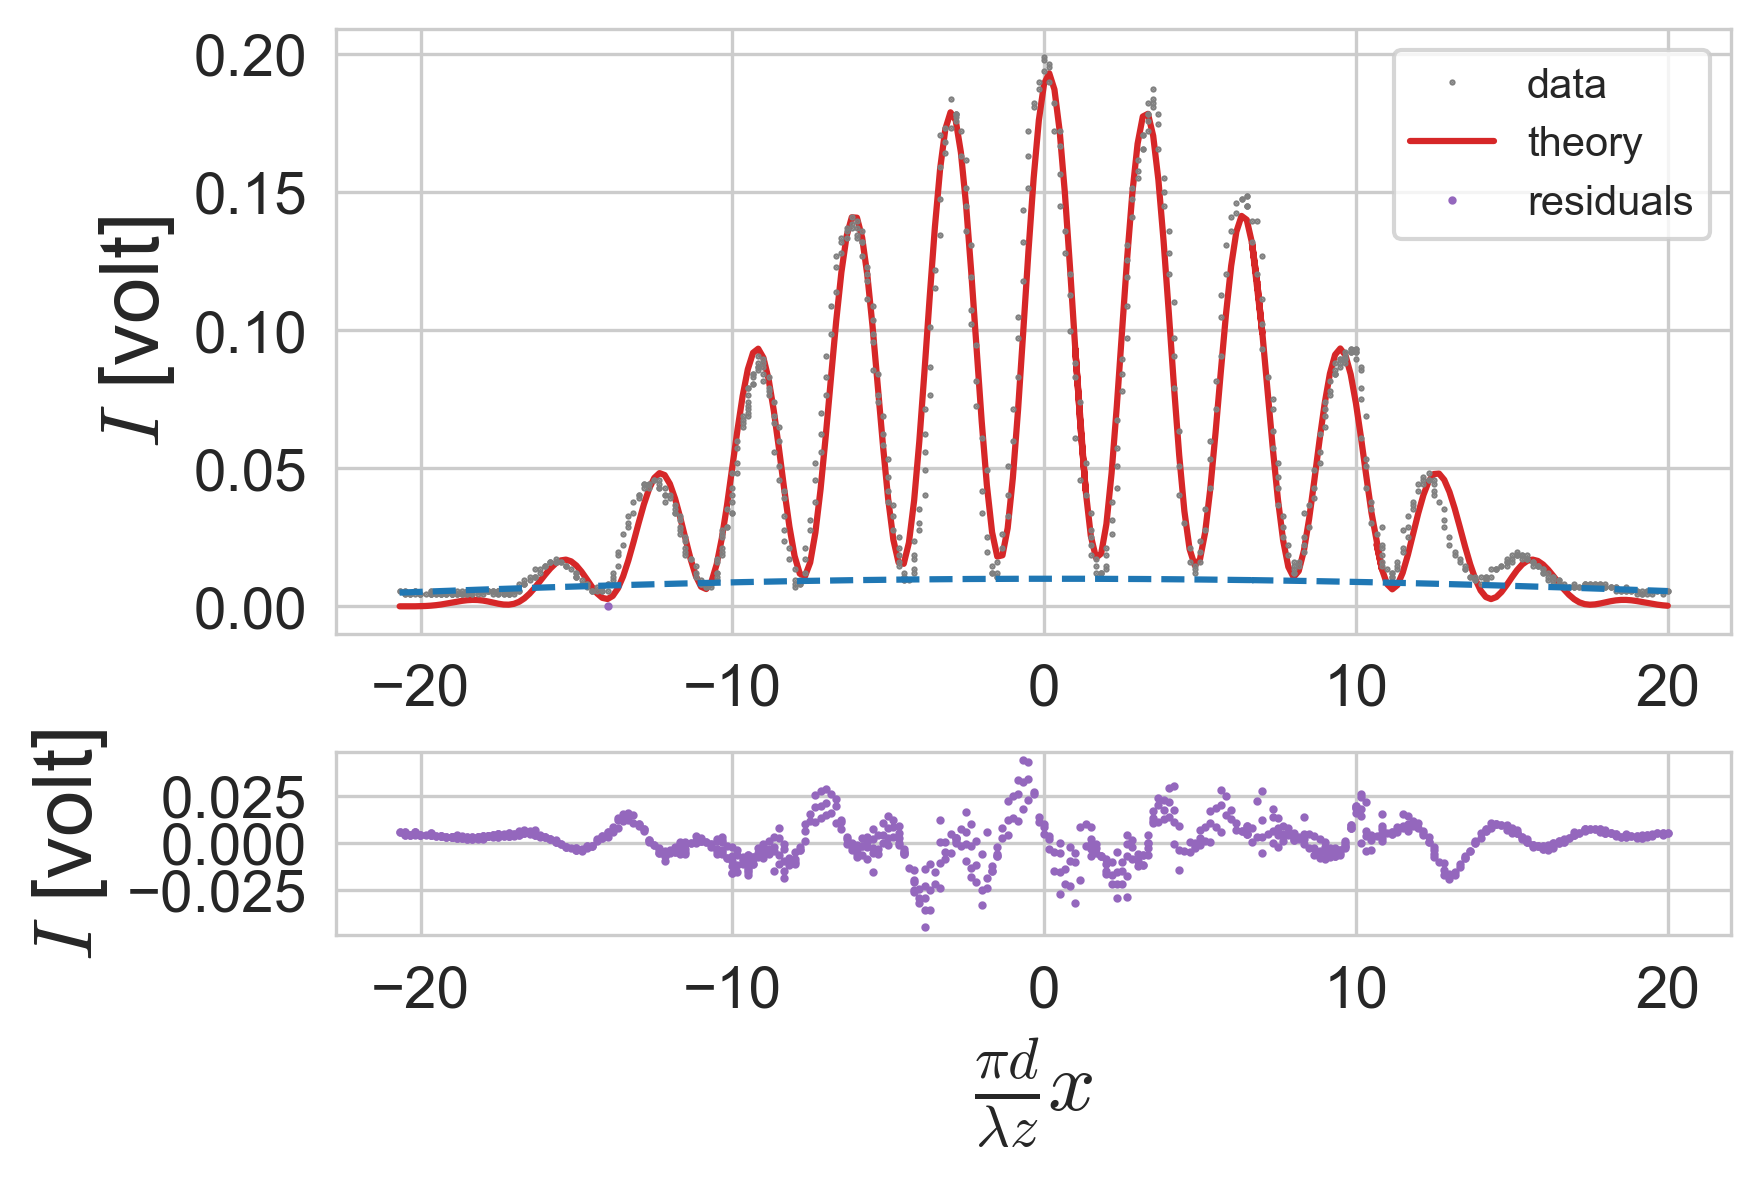
\includegraphics[width=0.9\columnwidth]{figures/0.04w0.25s memory.png}
    \caption{The secondary effects caused by measuring method are demonstrated here by the blue dashed line, we never see 0 intensity contrary to theory, and the visible offset in the fit relative to measurements. $(\sigma\sim0.01)$)}
    \label{fig:0.04w0.25s_memory}
\end{figure}
After taking into consideration the iris effect, our model describes our measurements with an error of $\sigma\sim0.01 $
(Where $\sigma$ was defined as the STD of the residuals),
The local minima seem to increase in value closer to $x=0$, and we are able to predict the general shape of the diffraction.
We also see an offset between theory and experiment that is, especially around the tails, one-sided.
We believe that tendency towards a certain side is duo to the fact that we scanned in a certain direction and the photoelectric sensor's measurement has a certain relaxation time which is not included in our model.

\begin{figure}[H]
    \centering
    \begin{subfigure}{0.5\columnwidth}
        \centering
        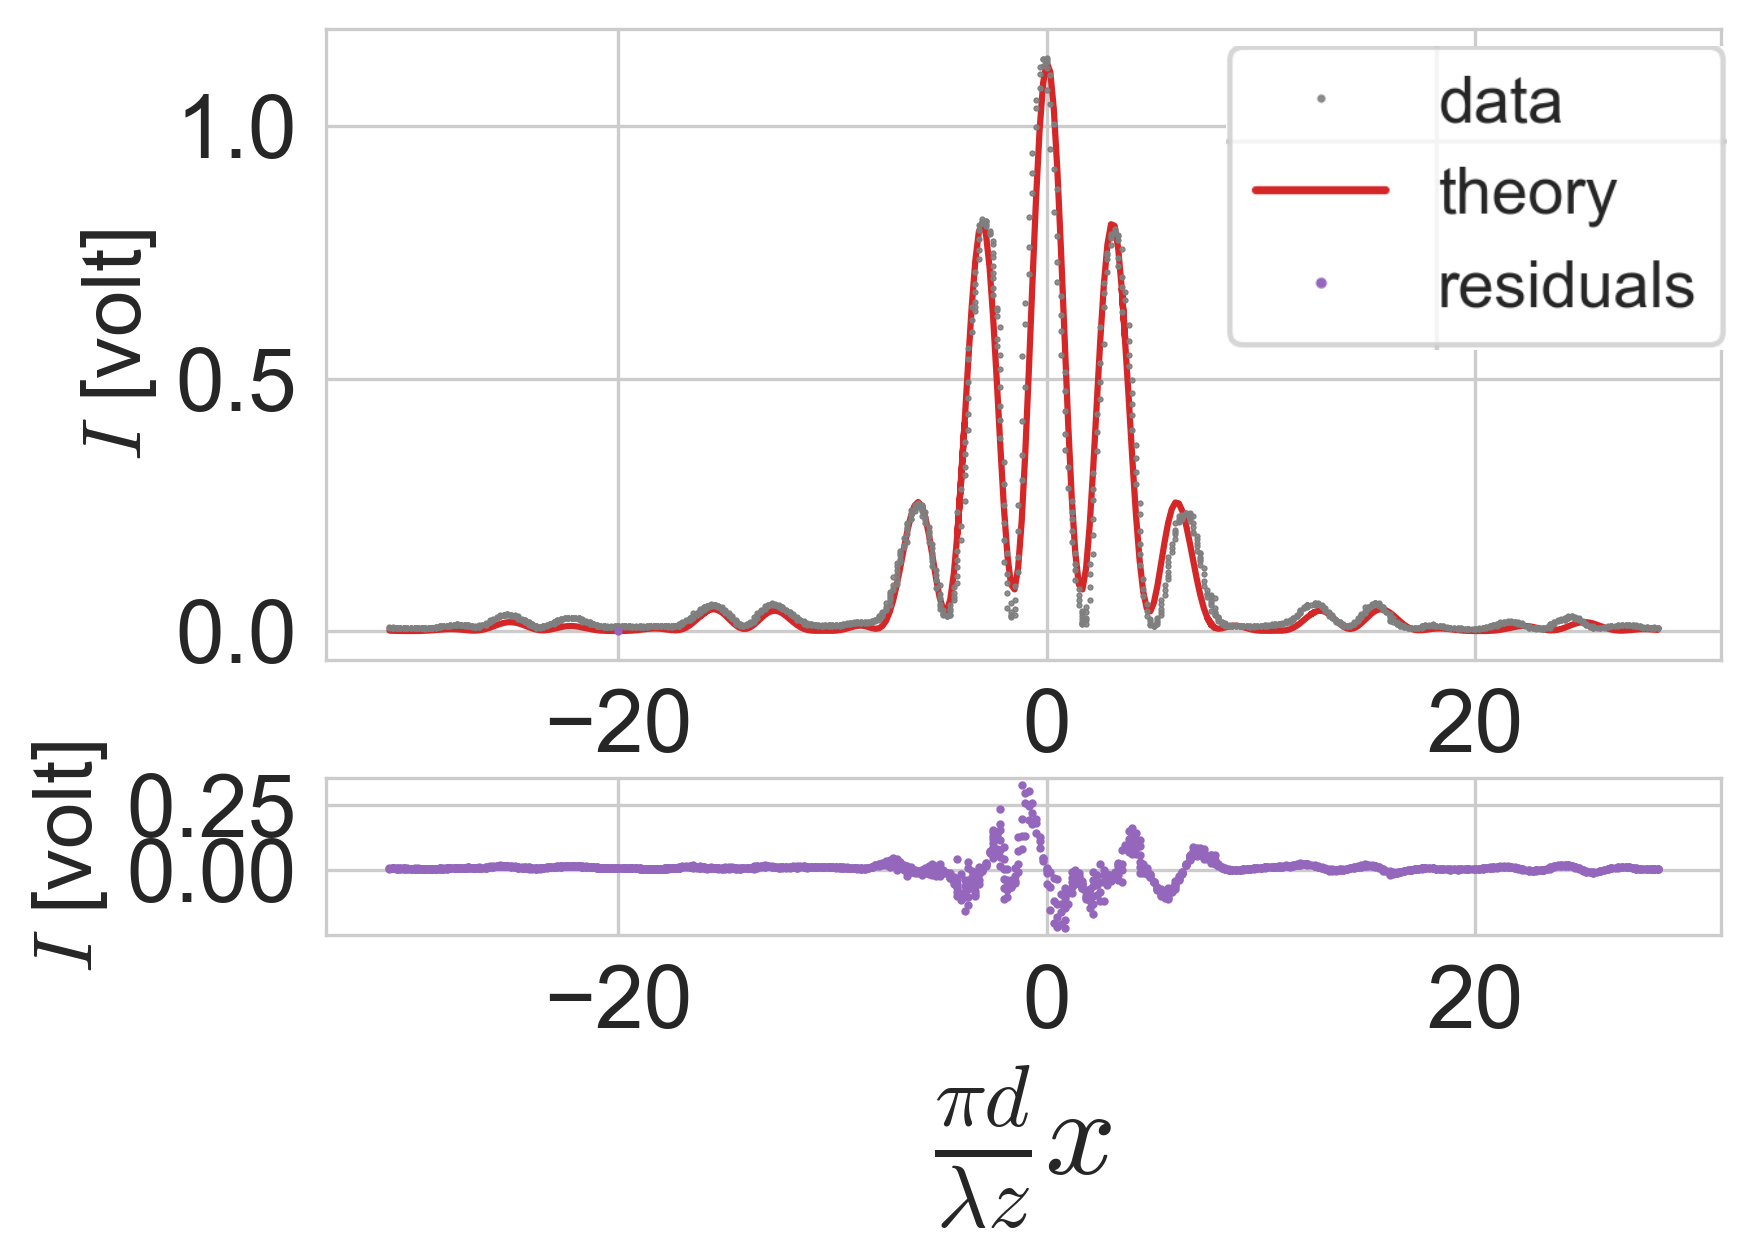
\includegraphics[width=\columnwidth]{figures/0.08w0.25s.png} % first figure itself
        \caption{\\$L=0.25[mm],d=0.08[mm]$}
        \label{fig:double slit interference 0.08w0.25s}
    \end{subfigure}\hfill
    \begin{subfigure}{0.5\columnwidth}
        \centering
        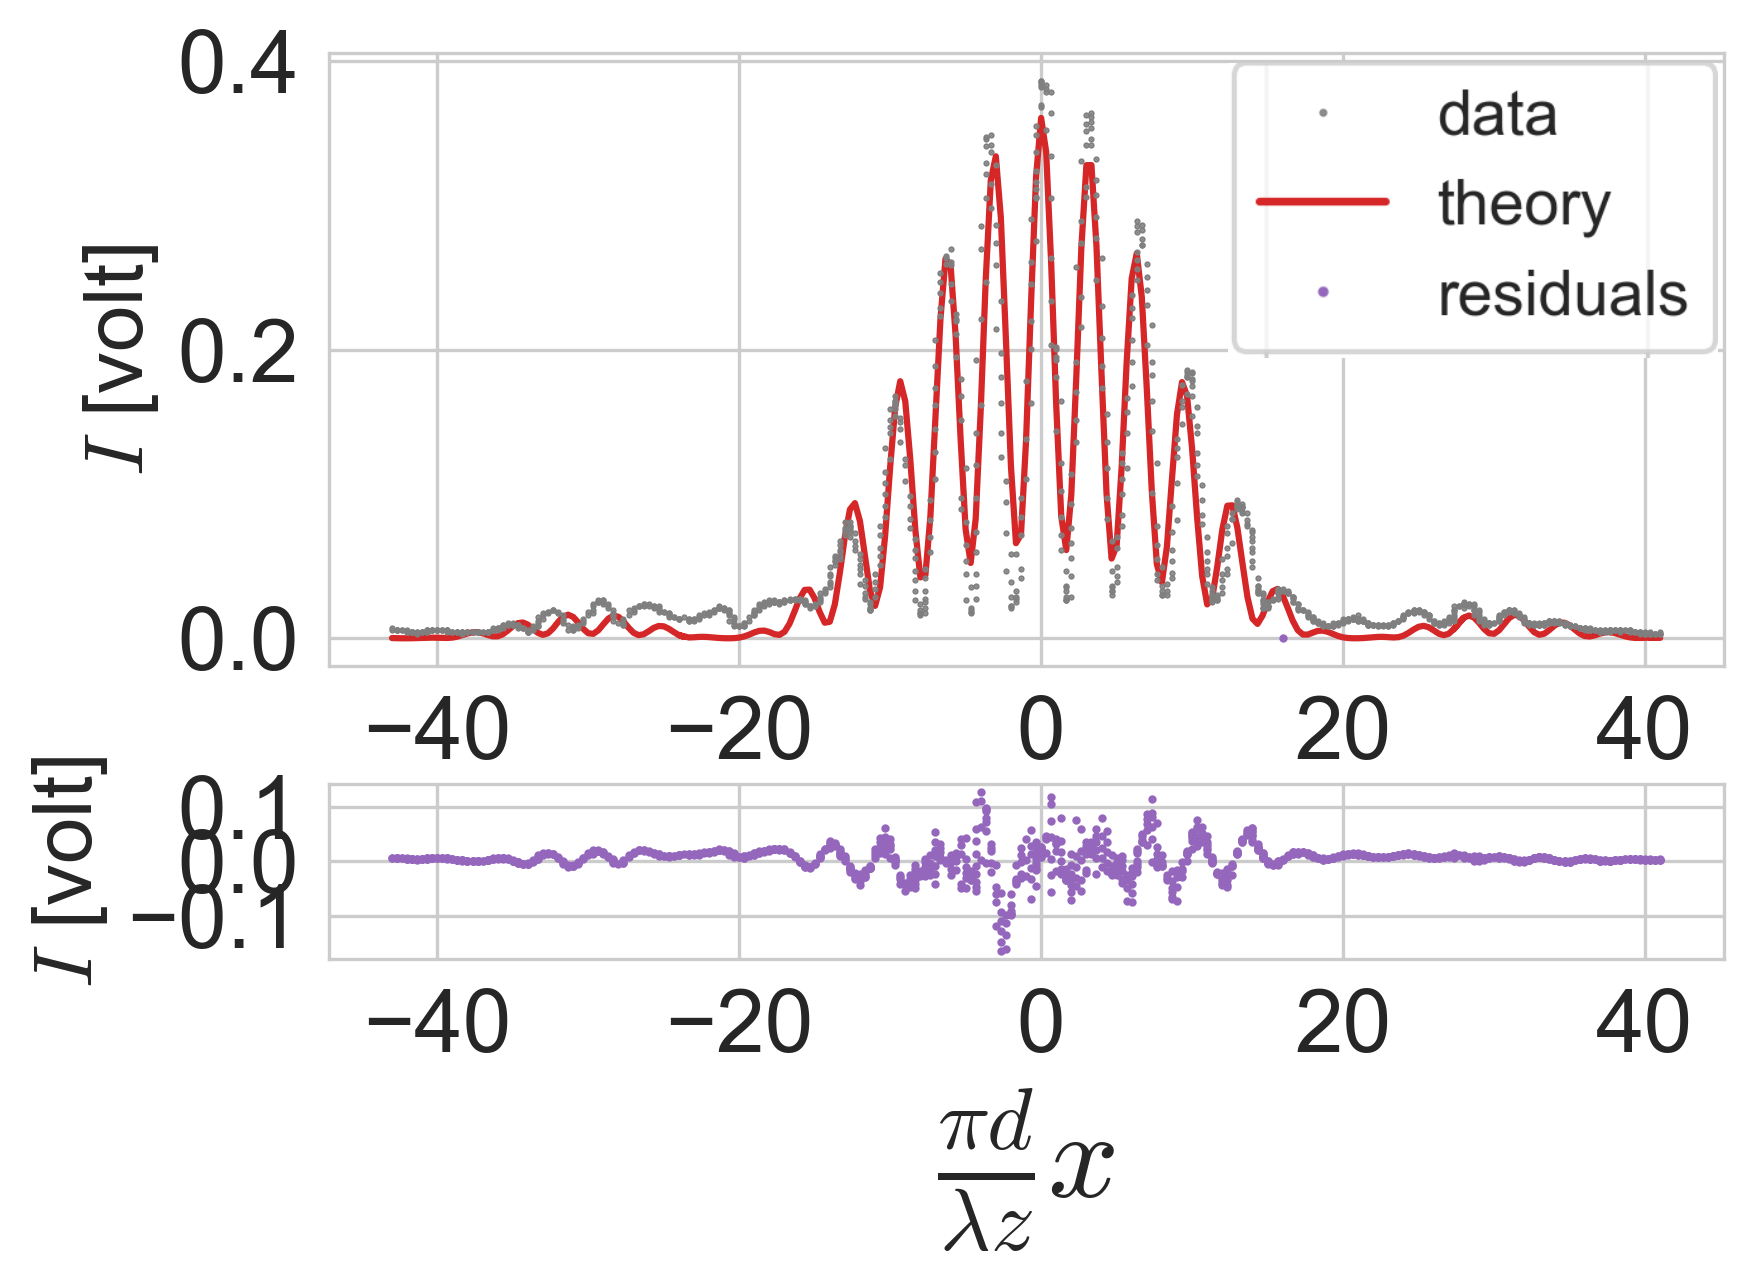
\includegraphics[width=\columnwidth]{figures/0.08w0.5s.png} % second figure itself
        \caption{\\$L=0.5[mm],d=0.08[mm]$}
        \label{fig:double slit interference 0.080.5s}
    \end{subfigure}
    \caption{Diffraction patterns for different slit patterns, for wider slits we get a narrow envelope of main peaks and for greater spacing we see denser peaks.}
    \label{other doubles}
\end{figure}

As seen in Figure \ref{other doubles}, when increasing the width of each slit the $sinc$ function is narrower, and for greater spaces between slits we see the increase in the $cos$ function's frequency as expected.
However, there's a change in amplitude upon changing $L$, contrary to what we'd predict.
That change comes from the fact we centered our laser beam between the slits, by measuring two positions of the slit for which we measure maximum amplitude then setting the beam between those, and greater distance between the slits means smaller initial amplitude for our plain wave.


